\section{Experimentos y Resultados} \label{sec:results}

\subsection{Configuración Experimental} \label{sec:results:setup}

Para evaluar la efectividad de NSGA-II en la estimación del parámetro de regularización \( \lambda \), los experimentos se realizaron utilizando datos sintéticos generados según el modelo de espacio de estados lineales descrito en la Sección \ref{sec:lit:two}. Se analizaron diferentes niveles de ruido \( \sigma \) (\( \sigma = 0, 0.05, 0.1 \)) para simular condiciones realistas de medición.

El proceso experimental incluyó:
\begin{enumerate}
    \item Resolución del problema de reconstrucción utilizando el método de la curva L para determinar \( \lambda \).
    \item Uso de NSGA-II para explorar un frente de Pareto de soluciones multi-objetivo considerando:
    \begin{itemize}
        \item \( \| \mathbf{y} - \mathbf{H} \mathbf{d} \|_2^2 \): Fidelidad de los datos,
        \item \( \| \mathbf{d} \|_2^2 \): Regularización,
        \item Penalización de negatividad: Para garantizar soluciones físicamente significativas.
    \end{itemize}
    \item Reconstrucción del perfil de absorción \( \mathbf{\mu} \) utilizando los valores de \( \lambda \) generados.
    \item Comparación gráfica y cuantitativa entre los resultados obtenidos con ambos métodos.
\end{enumerate}

\subsection{Resultados del Frente de Pareto} \label{sec:results:pareto}

El frente de Pareto generado por NSGA-II proporciona un conjunto de soluciones que representan diferentes compromisos entre los objetivos definidos. La Figura \ref{fig:pareto_front} muestra el frente de Pareto obtenido para \( \sigma = 0.05 \), donde cada punto representa un valor de \( \lambda \) y su correspondiente reconstrucción de \( \mathbf{d} \).

\begin{figure}[h]
    \centering
    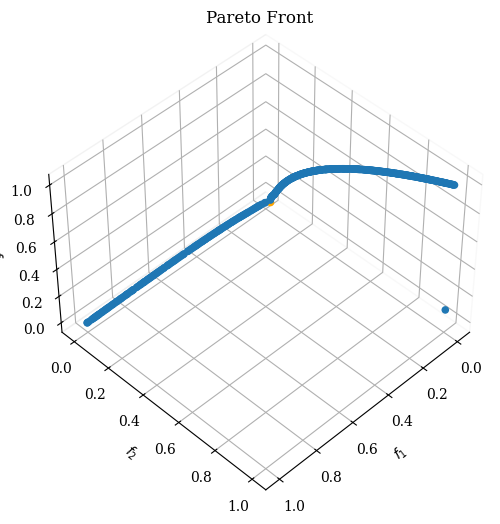
\includegraphics[width=0.8\textwidth]{pareto_front_single_value.png}
    \caption{Frente de Pareto generado por NSGA-II para \( \lambda \). El punto naranja representa la solución obtenida mediante la curva L.}
    \label{fig:pareto_front}
\end{figure}

Los resultados destacan que NSGA-II permite explorar soluciones más diversas que las proporcionadas por un único \( \lambda \) calculado mediante la curva L. Esto facilita la selección de soluciones óptimas adaptadas a restricciones específicas del problema.

\subsection{Comparación entre NSGA-II y la Curva L} \label{sec:results:comparison}

En esta sección se evalúan las soluciones obtenidas mediante NSGA-II y se comparan con la solución propuesta por la curva L. La Tabla \ref{tab:comparison} resume los valores de los objetivos normalizados para ambas metodologías.

\begin{table}[h]
    \centering
    \begin{tabular}{lccc}
        \toprule
        Método & Fidelidad (\( f_1 \)) & Regularización (\( f_2 \)) & Negatividad (\( f_3 \)) \\
        \midrule
        NSGA-II (mejor solución) & 0.XX & 0.XX & 0.XX \\
        Curva L & 0.XX & 0.XX & N/A \\
        \bottomrule
    \end{tabular}
    \caption{Comparación de las métricas entre NSGA-II y la curva L.}
    \label{tab:comparison}
\end{table}

Los resultados indican que, si bien la curva L proporciona una solución razonable, NSGA-II permite una exploración más amplia de \( \lambda \), lo que resulta en una mejor comprensión de los compromisos entre fidelidad y regularización.

\subsection{Reconstrucción del Perfil de Absorción \( \mathbf{\mu} \)} \label{sec:results:reconstruction}

La Figura \ref{fig:reconstruction_profiles} presenta los perfiles de absorción \( \mathbf{\mu} \) reconstruidos utilizando los valores de \( \lambda \) obtenidos mediante ambos métodos.

\begin{figure}[h]
    \centering
    \includegraphics[width=0.8\textwidth]{reconstruction_profiles.png}
    \caption{Perfiles de absorción \( \mathbf{\mu} \) reconstruidos. La curva azul corresponde a NSGA-II, mientras que la roja representa la solución de la curva L.}
    \label{fig:reconstruction_profiles}
\end{figure}

Aunque la curva L proporciona una solución única, NSGA-II permite seleccionar \( \lambda \) basándose en objetivos adicionales, como la penalización de negatividad, lo que resulta en perfiles físicamente más consistentes.

\subsection{Análisis de Correlación entre Objetivos} \label{sec:results:correlation}

Para interpretar los compromisos entre los objetivos, se analizó la correlación entre ellos. La Figura \ref{fig:correlation_matrix} muestra la matriz de correlación entre \( f_1 \), \( f_2 \) y \( f_3 \).

\begin{figure}[h]
    \centering
    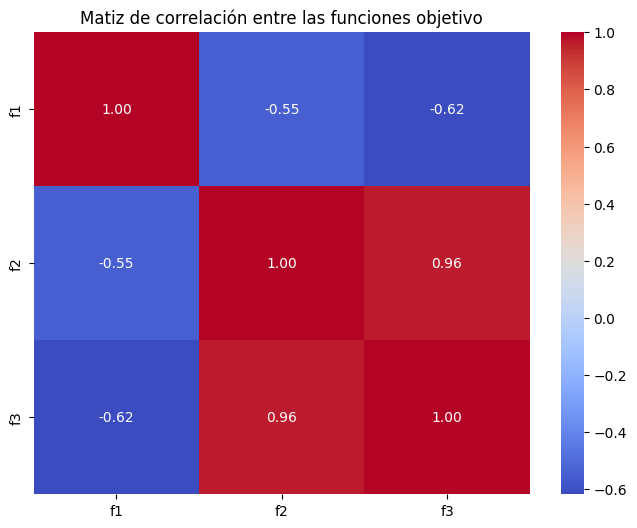
\includegraphics[width=0.7\textwidth]{correlation_matrix.png}
    \caption{Matriz de correlación entre los objetivos \( f_1 \), \( f_2 \) y \( f_3 \).}
    \label{fig:correlation_matrix}
\end{figure}

Los resultados destacan que \( f_1 \) y \( f_2 \) están altamente correlacionados, mientras que \( f_3 \) muestra una correlación negativa con \( f_1 \), indicando que minimizar negatividad puede comprometer ligeramente la fidelidad de los datos.

\subsection{Impacto del Nivel de Ruido} \label{sec:results:noise}

Los experimentos realizados con diferentes niveles de ruido (\( \sigma = 0, 0.05, 0.1 \)) resaltan la robustez de NSGA-II frente al ruido. A medida que \( \sigma \) aumenta, el frente de Pareto se desplaza, reflejando soluciones con menor fidelidad y mayor regularización. La Figura \ref{fig:pareto_noise} muestra cómo el nivel de ruido afecta el frente de Pareto.

\begin{figure}[h]
    \centering
    \includegraphics[width=0.8\textwidth]{pareto_front_noise.png}
    \caption{Efecto del nivel de ruido (\( \sigma \)) en el frente de Pareto.}
    \label{fig:pareto_noise}
\end{figure}

\subsection{Discusión de los Resultados} \label{sec:results:discussion}

Los resultados obtenidos sugieren que NSGA-II proporciona una metodología flexible y eficaz para explorar \( \lambda \) en la regularización de Tikhonov. Comparado con la curva L, NSGA-II ofrece:
\begin{itemize}
    \item Un conjunto diverso de soluciones que representan diferentes compromisos entre objetivos.
    \item Una mayor capacidad para incorporar restricciones adicionales, como la positividad de las soluciones.
    \item Una herramienta útil para analizar la sensibilidad del modelo frente al nivel de ruido.
\end{itemize}
